\documentclass{beamer}
\usepackage[latin1]{inputenc}
\usepackage{listings}
\usepackage{MnSymbol}
\usepackage{caption}
\usepackage{subcaption}
\usepackage{booktabs}

\DeclareMathAlphabet\mathbb{U}{msb}{m}{n}


\usetheme{Madrid}
\usecolortheme{beaver}
\title[Engineering Specifications and Mathematics]{Engineering Specifications and Mathematics\\for Verified Software}
\author{Hampton Smith}
\institute{Clemson University}
\date{May 16th, 2013}

\lstset{
	escapeinside={[*}{*]},
	basicstyle=\tiny
}

\lstdefinelanguage{Coq}
	{
		morekeywords={Definition,forall,let,Prop,Function,measure,if,then,else,end,match,with,unfold,intro,elim,reflexivity,replace,simpl,intros,split,change,rewrite,omega,assumption,symmetry,apply,auto,Qed,Theorem,functional,induction,in},
		sensitive=true,
		morecomment=[l]{--},
	}

\lstdefinelanguage{resolve}
	{
		morekeywords={restores,of,If,Recursive,Implicit,Powerset,Instance_Of,Theory,Precis,Categorical,introduces,related,Goal,Given,Definition,Facility,is,realized,by,Var,Concept,uses,Defines,Constraints,Initialization,Type,Family,exemplar,initialization,finalization,ensures,Operation,updates,requires,preserves,clears,evaluates,type,Extension,for,end,if,then,replaces,Procedure,convention,correspondence,iff,extended,Enhancement,Realization,represented,alters,in,modeled,constraint,While,changing,maintaining,decreasing,do,Theorem,For,all,implies,where,and,Precis,Subsumption},
		sensitive=true,
		morecomment=[l]{--},
		morecomment=[s]{(*}{*)},
		morestring=[b]",
	}
\lstset{language=resolve}


\begin{document}


\AtBeginSection[]
{
  \begin{frame}<beamer>
    \frametitle{Layout}
    \tableofcontents[currentsection,currentsubsection]
  \end{frame}
}


\begin{frame}
\titlepage
\end{frame}

\section{Introduction}
\begin{frame}{What is verified software?}
	\begin{itemize}
		\item Mathematically prove properties of a program
		\begin{itemize}
			\item No null dereferences
			\item No buffer overflows
			\item No deadlock
			\item Termination
			\item Full behavior
		\end{itemize}
		\item Requires formal semantics
		\item Description of the desired behavior in a formal language
		\item Can be demonstrated by hand or mechanically
	\end{itemize}
\end{frame}


\begin{frame}{How do we verify?}
	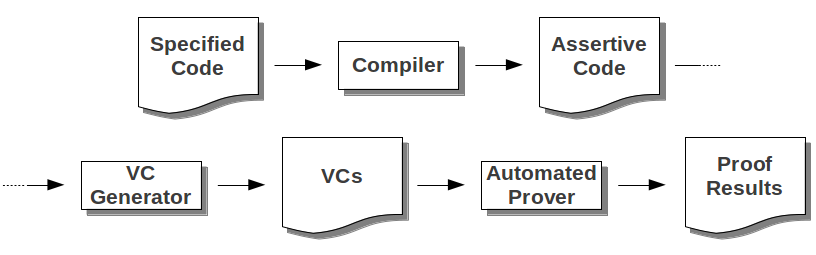
\includegraphics[width=\textwidth]{verification_pipeline}
\end{frame}


\subsection{Example Systems}
\begin{frame}{Example Systems}
	\begin{columns}
	\begin{column}[l]{5cm}
		Practical Systems
		\begin{itemize}
			\item Existing industrial languages (C, Java)
			\item Limited mathematical language
			\item Focus on verifying narrow properties
			\item Automatic proofs
		\end{itemize}
	\end{column}
	\begin{column}[r]{5cm}
		Pure Systems
		\begin{itemize}
			\item Research or pure mathematical language
			\item Rich mathematical language
			\item Full verification (up to termination)
			\item Interactive proofs
		\end{itemize}
	\end{column}
	\end{columns}
\end{frame}

\begin{frame}{Practical: Jahob}
	\begin{itemize}
		\item Implementation in a subset of Java
		\begin{itemize}
			\item No generics
			\item No dynamic dispatch
		\end{itemize}
		\item Specification in Isabelle
		\item Targets multiple back-end provers using intermediate first-order VC language
		\begin{itemize}
			\item CVC3
			\item Z3
		\end{itemize}
	\end{itemize}
\end{frame}


\begin{frame}
	\lstinputlisting[basicstyle=\tiny,language=Java]{ArrayList1.java}
\end{frame}


\begin{frame}{The Good and the Bad}
	\begin{itemize}
		\item Used to verify suite of linked data structures
		\item How does Jahob do it?
		\begin{itemize}
			\item Flexible, integrated specification tools
			\begin{itemize}
				\item Pre-/Post-conditions
				\item Auxiliary variables
				\item Concept definitions
			\end{itemize}
			\item Encourages first-order specs to target multiple provers
			\item Permits in-line hints
		\end{itemize}
		\item But, there are some problems...
		\begin{itemize}
			\item Complex proof obligations
			\item Lack of mathematical modularity
		\end{itemize}
	\end{itemize}
\end{frame}


\begin{frame}{Complex Proof Obligations}
	\begin{itemize}
		\item Must capture full Java complexity
		\begin{itemize}
			\item Null references
			\item Object aliasing
		\end{itemize}
		\item In-line assertions raise additional obligations
		\item Encourages cumbersome mathematical model
		\begin{itemize}
			\item Set of (index, element)
			\item Verify that no index appears twice
		\end{itemize}
	\end{itemize}
\end{frame}


\begin{frame}{Lack of Mathematical Modularity}
	\begin{itemize}
		\item Higher-order mathematics hamstrung
		\begin{itemize}
			\item Encouraged to use a subset of Isabelle's power
			\item Lack of generics/dynamic dispatch limit usefulness
			\begin{itemize}
				\item No way to parameterize a spec
				\item No way to pass a definition
			\end{itemize}
		\end{itemize}
		\item Coupling of specifications
	\end{itemize}
\end{frame}


\begin{frame}{Pure: Coq}
	\begin{itemize}
		\item Pure mathematical language based on the calculus of inductive constructions
		\item Provides its own functional implementation language
		\begin{itemize}
			\item OCaml
			\item Haskell
			\item Scheme
		\end{itemize}
		\item Emphasizes interactive proving
	\end{itemize}
\end{frame}


\begin{frame}
	\lstinputlisting[basicstyle=\scriptsize,language=Coq]{DivPred.coq}
	\lstinputlisting[basicstyle=\scriptsize,language=Coq]{DivImpl.coq}
	\lstinputlisting[basicstyle=\scriptsize,language=Coq]{DivTheorem.coq}
\end{frame}


\begin{frame}
	\lstinputlisting[basicstyle=\scriptsize,language=Coq]{DivProof.coq}
\end{frame}

\begin{frame}{The Good and the Bad}
	\begin{itemize}
		\item Been used to verify a C compiler
		\item How does Coq do it?
		\begin{itemize}
			\item Rich, extensible mathematical language
			\begin{itemize}
				\item Hierarchy of types
				\item Higher-order logic
				\item User-defined theories
			\end{itemize}
			\item Programming model is functional
			\item Exploits human intuitions
		\end{itemize}
		\item But, there are some problems...
		\begin{itemize}
			\item Poorly integrated with the programming realm
			\begin{itemize}
				\item Verify cases that can't happen!
			\end{itemize}
			\item Automated prover is more flexible, but slower
			\item No notion of programming components
			\begin{itemize}
				\item Next compiler must be verified from scratch
			\end{itemize}
		\end{itemize}
	\end{itemize}
\end{frame}


\begin{frame}{Best of Both Worlds?}
	\begin{itemize}
		\item Practical Systems
		\begin{itemize}
			\item Flexible, integrated specification
			\item Component support
		\end{itemize}
		\item Pure Systems
		\begin{itemize}
			\item Protection from certain complications (preferably still with the flexibility to use them)
			\item Rich, extensible mathematical language
		\end{itemize}
	\end{itemize}
\end{frame}

\subsection{Problem/Thesis Statement}
\begin{frame}{Problem Statement}
	\begin{itemize}
		\item Architecture and implementation of a minimalist rewrite prover to explore those prover capabilities practically necessary to mechanically verify well-engineered, modular components.
		\item Design and implementation of an extensible, flexible supporting mathematical framework for a practical verification system that permits reuse as well as the development of a rich set of models and assertions.
		\item Design and implementation of a well-integrated specification framework that is explicitely designed to work with the mathematical system, supporting verifiability by allowing simple, flexible specifications and supporting scalability by encouraging verified component reuse.
		\item Validation of our central hypothesis via application of the minimalist prover to software constructed using the mathematical and specification framework.
	\end{itemize}
\end{frame}

\begin{frame}{Dissertation Goal}
	In a verification system, an extensible, flexible mathematics and specification subsystem enables better-engineered component specifications and thus more straightforward proof obligations that are easily dispatched by even minimalistic automated provers.  Design, development, and experimentation with such a verification system is the goal of this dissertation.
\end{frame}


\section{Minimalist Prover}

\subsection{Design}
\begin{frame}{Minimalist Prover: Motivation}
	\begin{itemize}
		\item Prover is the final phase of the verification pipeline
		\item Sole determiner of which VCs can or can not be automatically proved
		\item Nearly all verification efforts focused on more efficient provers
		\item Our hypothesis suggests that, in many cases, \emph{flexibility} may trump raw performance
	\end{itemize}
\end{frame}

\begin{frame}{Minimalist Prover: Contributions}
	\begin{itemize}
		\item We demonstrate how a number of components can be engineered in a rigorous style to ease the verification process
		\item We experiment with a suite of prover heuristics intended to expose the programmer's underlying logic
		\item We confirm empirically that well-designed components built on an expressive mathematical framework can be dispatched by a minimalist prover
		\item Among these components, we present a mechanically verified generic sorting algorithm---a first
		\item For full details, see Chapter 7
	\end{itemize}
\end{frame}

\begin{frame}{Minimalist Prover: Design}
	\begin{itemize}
		\item Simple rewrite prover
		\item New features only when justified by VCs from real verification problems
		\item Flexible for experimentation
		\item Data collection for comparison
		\item Pedagogical deployments
	\end{itemize}
\end{frame}


\begin{frame}{Demo: Reversing a Queue}
~
\end{frame}


\begin{frame}{Automated Prover Algorithm}
	\begin{enumerate}
		\item Expand variables\\
			\texttt{i = j - 1}
		\item Develop antecedent\\
			\texttt{A and (A implies B) implies B}
		\item Explore consequent\\
		\begin{itemize}
			\item Tethered depth-first search\\
				Prevents \texttt{i = i + 1} or \texttt{Reverse(Empty\_String) = Empty\_String} from being applied ad nausium
			\item Terminates when proof space is exhausted or all consequents are dispatched
		\end{itemize}
	\end{enumerate}
\end{frame}


\begin{frame}{Automated Prover Algorithm}
	\begin{itemize}
		\item Extremely straightforward
		\item Closely mimics how a human mathematician might perform a proof
		\item Many irrelevant antecedent developments are likely to be made
		\item Antecedent development happens once, up-front, so time is less of an issue, but space complexity is combinatorial
		\item During consequent exploration, full proof space must be searched.  Combinatorial time complexity is a problem.
	\end{itemize}
\end{frame}


\begin{frame}{Automated Prover Algorithm: Heuristics}
	\begin{itemize}
		\item Detect and avoid useless transformations\\
			\texttt{S} $\rightarrow$ \texttt{S o Empty\_String}
		\item Develop only about relevant terms\\
			\texttt{f(a) and g(b) implies h(b)}
		\item Diversify givens
		\item Minimize as a preprocessing step
		\item Detect cycles
		\item Prioritize transformations as a preprocessing step\\
			\begin{enumerate}
				\item Reduce unique symbols
				\item Reduce function applications
			\end{enumerate}
	\end{itemize}
\end{frame}


\subsection{Evaluation}
\begin{frame}{Experimental Evaluation: Overview}
	\begin{itemize}
		\item Questions\\
		\begin{itemize}
			\item Is such a minimalist prover practical?
			\item Are the heuristics effective?
		\end{itemize}
		\item Approaches\\
		\begin{itemize}
			\item Series of verification benchmarks over multiple domains: integers, arrays, queues, trees
			\item Collect metrics
			\item How effective is the prover at dispatching VCs in a reasonable amount of time?
			\item What causes VCs not to prove?
			\item How does disabling each heuristic impact verification metrics?
		\end{itemize}
		\item For full details, see Chapter 6
	\end{itemize}
\end{frame}


\begin{frame}{Experimental Evaluation: Metrics}
	\begin{itemize}
		\item VCs proved
		\item Real time
		\item Operative steps
		\item Search steps (subset of operative steps occurring during consequent exploration)
	\end{itemize}
\end{frame}


\begin{frame}{Sorting a Queue}
	Specify a user-defined FIFO queue ADT that is generic (i.e., parameterized by the type of entries in a queue). Verify an operation that uses this component to sort the entries in a queue into some client-defined order.
	\vspace{2em}
	\lstinputlisting[language=resolve,caption=]{../proverEval/examples/Sorting_Capability.en}
\end{frame}


\begin{frame}{Sorting a Queue}
	\lstinputlisting[language=resolve,caption=]{examples/Selection_Sort_Realization1.rb}
\end{frame}


\begin{frame}{Sorting a Queue}
	\lstinputlisting[language=resolve,caption=]{examples/Selection_Sort_Realization2.rb}
\end{frame}


\begin{frame}{Sorting a Queue}
	\begin{itemize}
		\item VCs proved: 16/16
		\item Mean time: 1781
		\item Median proof steps: 8
		\item Median search steps: 0
		\item \textbf{XXX histogram XXX}
	\end{itemize}
\end{frame}


\begin{frame}{Demo: Array Realization of a Stack}
~
\end{frame}


\begin{frame}{Array Realization of a Stack}
	Specify a user-defined LIFO stack ADT that is generic (i.e., parameterized by the type of entries in a queue). Verify an array implementation of that ADT.
\end{frame}


\begin{frame}{Array Realization of a Stack}
	\lstinputlisting[language=resolve,caption=]{../proverEval/examples/Stack_Template.co}
\end{frame}


\begin{frame}{Array Realization of a Stack}
	\lstinputlisting[language=resolve,caption=]{examples/Array_Realiz.rb}
\end{frame}


\begin{frame}{Array Realization of a Stack}
	\begin{itemize}
		\item VCs proved: 27/27
		\item Mean time: 1707.1
		\item Median proof steps: 6
		\item Median search steps: 0
		\item \textbf{XXX histogram XXX}
	\end{itemize}
\end{frame}


\begin{frame}{Overall Experimentation Results}
	\begin{itemize}
		\item Six representative examples over integers, arrays, stacks, queues, and trees:\\
		\begin{itemize}
			\item Add/Multiply Integers
			\item Binary Search Array
			\item Sort a Queue
			\item Flip a Queue
			\item Array Implementation of Stack
			\item Modify and Restore a Tree
		\end{itemize}
		\item VCs proved: 127/133
		\item Mean time: 2493
		\item Median proof steps: 7
		\item Median search steps: 0
	\end{itemize}
\end{frame}


\begin{frame}{Overall Experimentation Results}
	\begin{figure}
		\centering
		\begin{subfigure}[b]{0.40\textwidth}
			\centering
			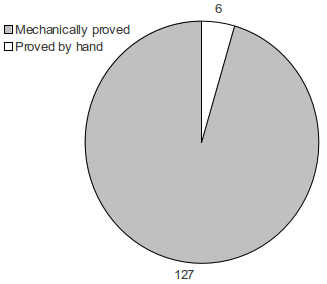
\includegraphics[width=\textwidth]{../proverEval/proofResults3.png}
			\caption{Verification results\label{fig:pie}}
		\end{subfigure}
		\quad
		\begin{subfigure}[b]{0.55\textwidth}
			\centering
			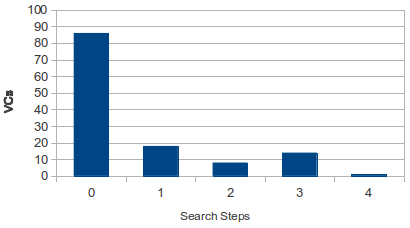
\includegraphics[width=\textwidth]{../proverEval/searchSteps2.png}
			\caption{Number of Search Steps Required by Proofs\label{fig:histogram}}
		\end{subfigure}
	\end{figure}
\end{frame}


\begin{frame}{Heuristic Evaluation}
	\tiny
	\begin{tabular}{lrrrrrrr}
		\toprule
			& $\sum \Delta\text{Proved}$	& $\overline{\Delta t / \sigma}$	& $\sum\Delta t$ & $\overline{\Delta\text{steps}}$ & $\sum\Delta\text{steps}$ & $\overline{\Delta\text{search}}$ & $\sum\Delta\text{search}$ \\
		\midrule
		With useless \\
		transformations		& -12	& 4.07	& 83438		& 0	& 0	& 0	& 0	\\
		\midrule
		Developing about \\
		irrelevant terms	& -1	& 8.80	& 154530	& 0	& 0	& 0	& 0\\
		\midrule
		Not checking for \\
		diversity of givens	& -6	& -5.55	& -142026	& -0.02	& -4	& -0.01	& -1	\\
		\midrule
		No minimization		& -10	& 2.53	& 36651		& 0.02	& 3	& 0.28	& 35	\\
		\midrule
		No cycle detection	& 0	& 0.60	& 9629		& 0.08	& 11	& 0.08	& 11	\\
		\midrule
		No prioritization \\
		of transformations	& -19	& 2.60	& 17577		& 0.05	& 6	& 0.04	& 5	\\
		\bottomrule
	\end{tabular}
\end{frame}

\section{Mathematical Flexibility}

\lstset{
	basicstyle=\footnotesize
}


\subsection{Design}
\begin{frame}{Mathematical Flexibility: Motivation}
	\begin{itemize}
		\item Mathematical system is the language of specification
		\item It is the source of an increase in effort for verified software
		\item Therefore, it needs to be familiar and its results reusable
		\item Pure systems contain many useful features that practical systems do not take advantage of
	\end{itemize}
\end{frame}

\begin{frame}{Mathematical Flexibility: Contributions}
	\begin{itemize}
		\item We demonstrate how a number of features from pure systems (higher-order definitions, first-class types, etc.) can be utilized to ease the verification task in a practical system
		\item We provide a mathematical foundation for several pre-existing RESOLVE features
		\item We introduce novel tools for static reasoning in the presence of dependent types
		\item For full details, see Chapter 5
	\end{itemize}
\end{frame}



\begin{frame}{Tools for Static Reasoning}
	\begin{itemize}
		\item First-class types permit undecidable type relationships
		\item Nonetheless, static typing is a useful tool
		\item \emph{Type theorems} are a novel compromise introduced by this research
	\end{itemize}
	\vspace{2em}
	\lstinputlisting[language=resolve,caption=]{examples/typeTheorem1.mt}
\end{frame}

\begin{frame}{Tools for Static Reasoning}
	\begin{figure}
		\centering
		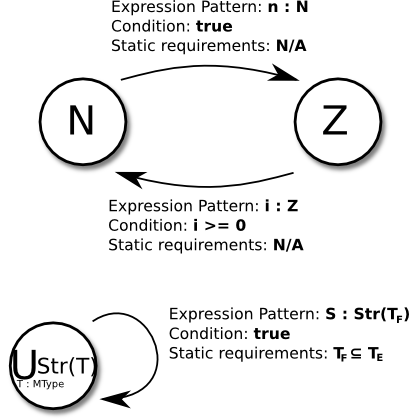
\includegraphics[width=.6\textwidth]{../typeGraph.png}
	\end{figure}
\end{frame}


\subsection{Evaluation}
\begin{frame}{Sorting a Queue}
	\lstinputlisting[basicstyle=\tiny,language=resolve,caption=]{../mathEval/examples/Sorting_Capability.en}
\end{frame}

\begin{frame}{Sorting a Queue}
	\lstinputlisting[basicstyle=\tiny,language=resolve,caption=]{../mathEval/examples/String_Theory1.mt}
\end{frame}

\begin{frame}{Sorting a Queue}
	\lstinputlisting[basicstyle=\tiny,language=resolve,caption=]{examples/String_Theory2.mt}
\end{frame}

\begin{frame}{Sorting a Queue}
	\lstinputlisting[basicstyle=\tiny,language=resolve,caption=]{../mathEval/examples/totalpreorderingvc.asrt}
\end{frame}

\begin{frame}{Sorting a Queue}
	\lstinputlisting[basicstyle=\scriptsize,language=resolve,caption=]{examples/preorderingTheorem.mt}
\end{frame}

\begin{frame}{Error Analysis and Reporting}
~
\end{frame}


\begin{frame}{Array Realization of a Stack}
	\lstinputlisting[basicstyle=\tiny,language=resolve,caption=]{../mathEval/examples/Array_Realiz1.rb}
\end{frame}

\begin{frame}{Array Realization of a Stack}
	\lstinputlisting[basicstyle=\tiny,language=resolve,caption=]{../mathEval/examples/Binary_Iterator_Theory1.mt}
\end{frame}

\begin{frame}{Error Analysis and Reporting}
~
\end{frame}


\begin{frame}{Classroom Experiment}
	\begin{itemize}
		\item Mathematical development assignment given to a graduate-level programming languages class for extra-credit
		\item Example demonstrating first-class types and type theorems
		\item No formal training
		\item Assignment asked increasingly difficult questions: last three required analysis and adaptation\\
		\begin{enumerate}
			\item Asserts that \texttt{Without\_Last\_Zero(10)~=~1}.  This may require an extra step to establish proper symbols.
			\item Asserts that for any multiple of ten, \texttt{t,~Next\_Even(t)~mod~10~=~2}.  This may require some additional steps to establish proper symbols and relationships.
			\item Asserts that for all multiples of ten, \texttt{t}, and integers, \texttt{i}, \texttt{Without\_Last\_Zero(t~*~i)~=~i}.  This may require some additional steps.
		\end{enumerate}
	\end{itemize}
\end{frame}

\begin{frame}{Classroom Experiment}
	\begin{itemize}
		\item 7/9 students participated
		\item All but one student successfully completed questions 10 and 11 correctly
		\item Two of the seven completed 12 correctly
	\end{itemize}
\end{frame}





\section{Conclusion}
\begin{frame}{Conclusion}
	\begin{itemize}
		\item Systems need not be limited to the features of a pure or a practical system. Our hybrid system incorporates features of practical verification systems (static checking, efficient implementation, polymorphism) with pure mathematical systems (dependent types, higher-order logic, mathematical reusability.)
		\item Novel mechanism for static reasoning can be used to bridge the gap between undecidable, but flexible type systems and constrained, hierarchical systems.
		\item It can be demostrated empirically that using such a language, a programmer is capable of creating components about which reasoning is sufficiently easy that VCs can be dispatched by a minimalist prover.
		\item This includes a verified generic sorting algorithm---a first.
		\item A variety of useful heuristics exist to help a minimalist prover expose programmer intuition.
	\end{itemize}
\end{frame}

\begin{frame}{Future Directions}
	\begin{itemize}
		\item Better transformation fitness functions
		\item Other prover styles
		\item Evaulate usability of new features
		\item Increase type-system intuitiveness
		\item Prover scalability
	\end{itemize}
\end{frame}


\begin{frame}{Questions?}
~
\end{frame}

\end{document}
